\section{Textos en Processing}

Para escribir un texto en Processing usaremos la función
\begin{center}
\texttt{text(string Texto,float X,float Y\color{gray}{[,float Z]}\color{black})}
\end{center}
que dibuja en pantalla. Muestra la información especificada en el primer párametro de sobre el área de trabajo en la 
posición indicada por los parámetros adicionales. A menos que se indique con la función \texttt{textFont()}, se usará 
una fuente con su tamaño predefinidos. El cambio de color del texto se puede hacer con \texttt{fill()}. De igual forma 
se mostrará el texto de acuerdo con la función \texttt{textAlign()}, permitiéndonos dibujar a la izquierda, a la 
derecha o al centro de las coordenadas.


%%%%%%%%%%%%%%%%%%%%%%
%      Ejemplo 1     %
%%%%%%%%%%%%%%%%%%%%%%
\mbox{\color{Brown}\begin{minipage}{.55\textwidth}%
        \VerbatimInput[fontsize=\scriptsize,frame=lines,label=Ejemplo 1: Diferentes formatos]{./ejemplo1/ejemplo1.pde}%
\end{minipage}}\hspace{.1\textwidth}
\mbox{\begin{minipage}{\textwidth}%
        
\includegraphics[width=.15\textwidth]{./ejemplo1.png}
\end{minipage}}

%%%%%%%%%%%%%%%%%%%%%%
%      Ejemplo 2     %
%%%%%%%%%%%%%%%%%%%%%%

\mbox{\color{Brown}\begin{minipage}{.55\textwidth}%
        \VerbatimInput[fontsize=\scriptsize,frame=lines,label=Ejemplo 2: Alejamiento mediante el parámetro %
\texttt{Z}]{./ejemplo2/ejemplo2.pde}%
\end{minipage}}\hspace{.1\textwidth}
\mbox{\begin{minipage}{\textwidth}%
        
\includegraphics[width=.15\textwidth]{./ejemplo2.png} 
\end{minipage}}

%%%%%%%%%%%%%%%%%%%%%%
%      Ejemplo 3     %
%%%%%%%%%%%%%%%%%%%%%%

\mbox{\color{Brown}\begin{minipage}{.55\textwidth}%
        \VerbatimInput[fontsize=\scriptsize,frame=lines,label=Ejemplo 3: Encerrando un texto en una caja %
\texttt{Z}]{./ejemplo3/ejemplo3.pde}%
\end{minipage}}\hspace{.1\textwidth}
\mbox{\begin{minipage}{\textwidth}%
        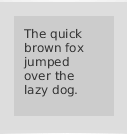
\includegraphics[width=.15\textwidth]{./ejemplo3.png} 
\end{minipage}}
